\documentclass[a4paper,11pt]{scrartcl}
\usepackage{mmap}
\usepackage[margin=1in]{geometry} % decreases margins
\usepackage{setspace}
\setlength{\parskip}{0pt}
\onehalfspacing

\usepackage{fontspec}
\usepackage{bold-extra}
\setmonofont[AutoFakeSlant=0.2,Scale=0.95]{D2Coding}
\setsansfont[BoldFont=AppleSDGothicNeo-SemiBold]{Apple SD Gothic Neo}
\setmainfont[AutoFakeSlant=0.2,BoldFont=SDMyeongjoNeoa-eSm,WordSpace={1.0,0.5,0.5},Kerning=On]{SDMyeongjoNeoa-bLt}

\usepackage{graphicx}
\usepackage{longfbox}
\usepackage{kotex}

\addtokomafont{labelinglabel}{\bfseries}
\addtokomafont{title}{\bfseries}

\setkomafont{disposition}{\normalfont}
\setkomafont{section}{\LARGE\bfseries\sffamily}
\setkomafont{subsection}{\Large\mdseries\sffamily}

\title{\vspace{-0.5in}LangComp HW5}
\author{\vspace{-15pt}2016-19986 정누리}
\date{\vspace{-5pt}\today}

%++++++++++++++++++++++++++++++++++++++++

\begin{document}

\maketitle

\section*{Code}
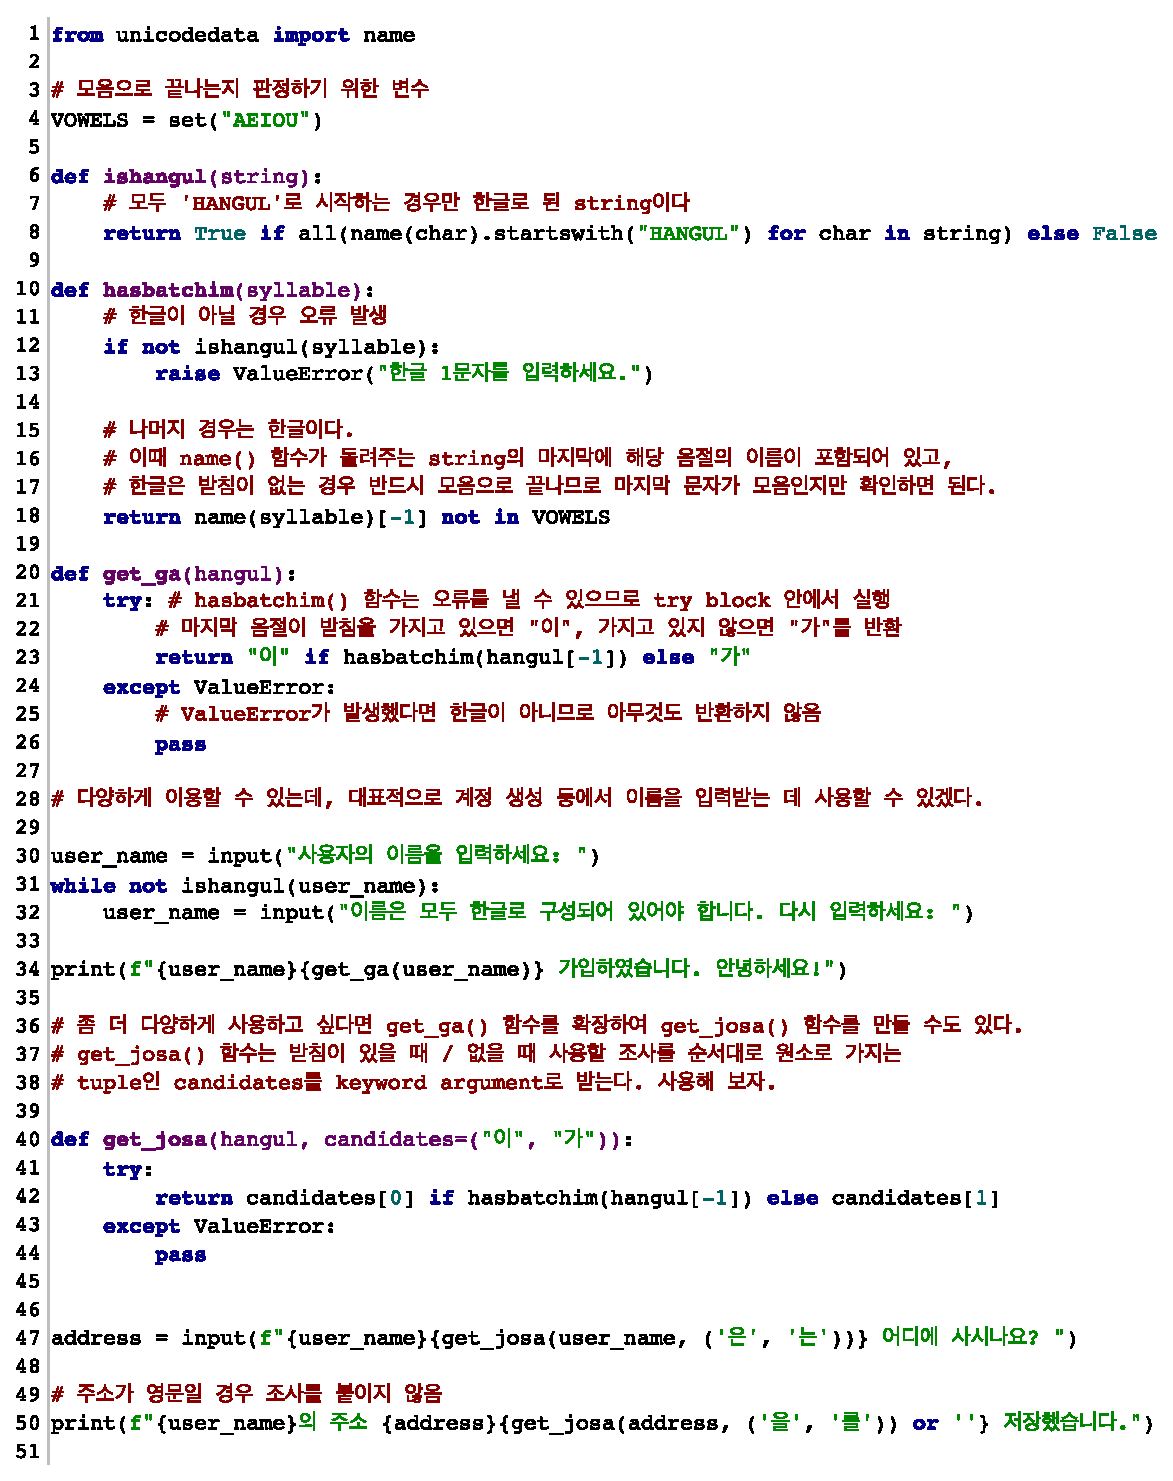
\includegraphics[height=18cm]{hw05.eps}

\section*{Tests}
한글이 아닌 이름을 입력하면 다시 묻는다.
\par\bigskip
\begin{longfbox}[margin-left=1em]
  \ttfamily
  사용자의 이름을 입력하세요: wjdsnfl \\
  이름은 모두 한글로 구성되어 있어야 합니다. 다시 입력하세요: 정누리 \\
  정누리가 가입하였습니다. 안녕하세요! \\
  정누리는 어디에 사시나요? 집 \\
  정누리의 주소 집을 저장했습니다.
\end{longfbox}

\par\bigskip\noindent
영문 주소에 대해서는 별도의 조사를 붙이지 않는다.

\par\bigskip
\begin{longfbox}[margin-left=1em]
  \ttfamily
  사용자의 이름을 입력하세요: 정누리 \\
  정누리가 가입하였습니다. 안녕하세요! \\
  정누리는 어디에 사시나요? home \\
  정누리의 주소 home 저장했습니다.
\end{longfbox}
\end{document}
